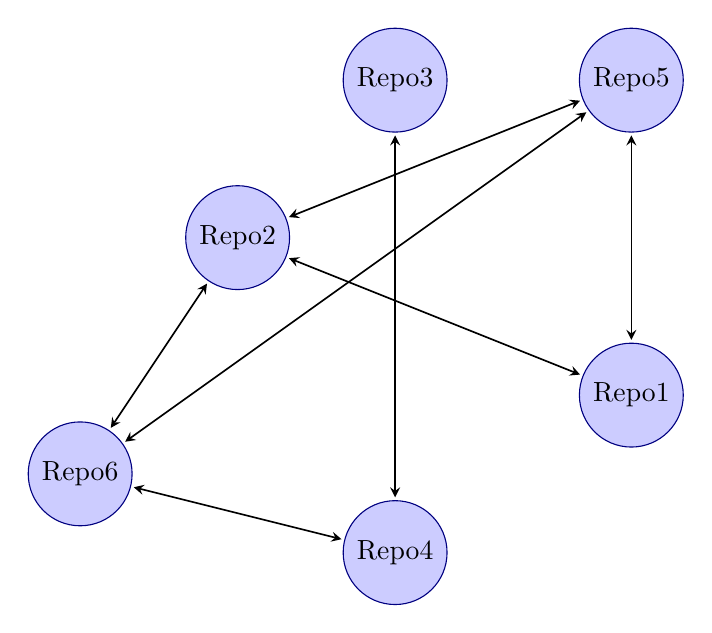
\begin{tikzpicture}
[repo/.style={circle,
		fill=green!20!white,
		draw=green!50!black,
		minimum size=10mm},
workingcopy/.style={circle,
		fill=blue!20!white,
		draw=blue!50!black,
		minimum size=5mm},
link/.style={<->, shorten <=1pt, shorten >=1pt, >=stealth, semithick}]

% central repo
%\node at (0, 0) [repo] (mainrepo) { Repository };
% working copies
\node at (3,-1)  [workingcopy] (repo1) { Repo1 };
\node at (-2,1)  [workingcopy] (repo2) { Repo2 };
\node at (0,3)   [workingcopy] (repo3) { Repo3 };
\node at (0,-3)  [workingcopy] (repo4) { Repo4 };
\node at (3,3)   [workingcopy] (repo5) { Repo5 };
\node at (-4,-2) [workingcopy] (repo6) { Repo6 };
% links between repos
\draw [link] (repo1) -- (repo2);
\draw [link] (repo1) -- (repo5);
\draw [link] (repo2) -- (repo5);
\draw [link] (repo3) -- (repo4);
\draw [link] (repo6) -- (repo2);
\draw [link] (repo6) -- (repo5);
\draw [link] (repo4) -- (repo6);
\end{tikzpicture}
